% Created 2021-07-04 Sun 19:39
% Intended LaTeX compiler: pdflatex
\documentclass[11pt]{article}
\usepackage[utf8]{inputenc}
\usepackage[T1]{fontenc}
\usepackage{graphicx}
\usepackage{grffile}
\usepackage{longtable}
\usepackage{wrapfig}
\usepackage{rotating}
\usepackage[normalem]{ulem}
\usepackage{amsmath}
\usepackage{textcomp}
\usepackage{amssymb}
\usepackage{capt-of}
\usepackage{hyperref}
\graphicspath{{../../books/}}
% TIPS
% \substack{a\\b} for multiple lines text





% pdfplots will load xolor automatically without option
\usepackage[dvipsnames]{xcolor}

\usepackage{forest}
% two-line text in node by [two \\ lines]
% \begin{forest} qtree, [..] \end{forest}
\forestset{
  qtree/.style={
    baseline,
    for tree={
      parent anchor=south,
      child anchor=north,
      align=center,
      inner sep=1pt,
    }}}
%\usepackage{flexisym}
% load order of mathtools and mathabx, otherwise conflict overbrace

\usepackage{mathtools}
%\usepackage{fourier}
\usepackage{pgfplots}
\usepackage{amsthm, mathabx,  amsmath, commath}
\usepackage{amsfonts}

\usepackage{empheq}
\usepackage{tikz}
\usetikzlibrary{arrows.meta}
\usepackage[most]{tcolorbox}

\newtheorem{theorem}{Theorem}[section]
\newtheorem{definition}{Definition}[section]
\newtheorem{corollary}{Corollary}[section]
\newtheorem{example}{Example}[section]
\newtheorem{lemma}{Lemma}[section]
\newtheorem{proposition}{Proposition}[section]

\newcommand{\bl}[1] {\boldsymbol{#1}}
\newcommand{\Wt}[1] {\stackrel{\sim}{\smash{#1}\rule{0pt}{1.1ex}}}
\newcommand{\wt}[1] {\widetilde{#1}}


%For boxed texts in align, use Aboxed{}
%otherwise use boxed{}

\DeclareMathSymbol{\widehatsym}{\mathord}{largesymbols}{"62}
\newcommand\lowerwidehatsym{%
  \text{\smash{\raisebox{-1.3ex}{%
    $\widehatsym$}}}}
\newcommand\fixwidehat[1]{%
  \mathchoice
    {\accentset{\displaystyle\lowerwidehatsym}{#1}}
    {\accentset{\textstyle\lowerwidehatsym}{#1}}
    {\accentset{\scriptstyle\lowerwidehatsym}{#1}}
    {\accentset{\scriptscriptstyle\lowerwidehatsym}{#1}}
}

\usepackage{graphicx}
    
% text on arrow for xRightarrow
\makeatletter
%\newcommand{\xRightarrow}[2][]{\ext@arrow 0359\Rightarrowfill@{#1}{#2}}
\makeatother


\def \bx {\boldsymbol{x}}
\def \ba {\boldsymbol{a}}
\def \bI {\boldsymbol{I}}
\def \bt {\boldsymbol{t}}
\def \bb {\boldsymbol{b}}
\def \bA {\boldsymbol{A}}
\def \bX {\boldsymbol{X}}
\def \bu {\boldsymbol{u}}
\def \bS {\boldsymbol{S}}
\def \bZ {\boldsymbol{Z}}
\def \bz {\boldsymbol{z}}
\def \by {\boldsymbol{y}}
\def \bw {\boldsymbol{w}}
\def \bT {\boldsymbol{T}}
\def \bS {\boldsymbol{S}}
\def \bm {\boldsymbol{m}}
\def \bW {\boldsymbol{W}}
\def \bY {\boldsymbol{Y}}
\def \bH {\boldsymbol{H}}
\def \blambda {\boldsymbol{\lambda}}
\def \bPhi {\boldsymbol{\Phi}}
\def \btheta {\boldsymbol{\theta}}
\def \bmu {\boldsymbol{\mu}}
\def \bphi {\boldsymbol{\phi}}
\def \bSigma {\boldsymbol{\Sigma}}
\def \lb {\left\{}
\def \rb {\right\}}
\def \caln {\mathcal{N}}
\def \dissum {\displaystyle\Sigma}
\def \dispro {\displaystyle\prod}
\def \E {\mathbb{E}}
\def \Q {\mathbb{Q}}
\def \V {\mathbb{V}}
\def \R {\mathbb{R}}
\def \calq {\mathcal{Q}}
\def \calg {\mathcal{G}}
\def \caln {\mathcal{N}}
\def \calr {\mathcal{R}}
\def \calm {\mathcal{M}}
\def \calc {\mathcal{C}}
\def \bcup {\bigcup}

\makeindex
\author{Rotman}
\date{\today}
\title{An Introduction To Algebraic Topology}
\hypersetup{
 pdfauthor={Rotman},
 pdftitle={An Introduction To Algebraic Topology},
 pdfkeywords={},
 pdfsubject={},
 pdfcreator={Emacs 27.2 (Org mode 9.5)}, 
 pdflang={English}}
\begin{document}

\maketitle
\tableofcontents


\section{Introduction}
\label{sec:org16bbfca}

\subsection{Notation}
\label{sec:org0e82024}
\(\bI=[0,1]\).
\begin{equation*}
S^n=\{x\in\R^{n+1}\mid\norm{x}=1\}
\end{equation*}
\(S^n\) is called the \textbf{\(n\)-sphere}. \(S^n\subset\R^{n+1}\) (\(S^1\) is the circle); 0-sphere \(S^0\)
consists of the two points \(\{-1,1\}\) and hence is a discrete two-point space. We may
regard \(S^n\) as the \textbf{equator} of \(S^{n+1}\)
\begin{equation*}
S^n=\R^{n+1}\cap S^{n+1}=\{(x_1,\dots,x_{n+2})\in S^{n+1}:x_{n+2}=0\}
\end{equation*}
The \textbf{north pole} is \((0,0,\dots,0,1)\in S^n\); the \textbf{south pole} is \((0,0,\dots,0,-1)\). The \textbf{antipode}
of \(x=(x_1,\dots,x_{n+1})\in S^n\) is the other endpoint of the diameter having one endpoint \(x\); thus
the antipode of \(x\) is \(-x=(-x_1,\dots,-x_{n+1})\), for the distance from \(-x\) to \(x\) is 2.
\begin{equation*}
D^n=\{x\in\R^n\mid\norm{x}\le 1\}
\end{equation*}
\(D^n\) is called the \textbf{\(n\)-disk} (or \textbf{\(n\)-ball}).  Observe that \(S^{n-1}\subset D^n\subset \R^n\);
indeed \(S^{n-1}\) is the boundary of \(D^n\) in \(\R^n\)
\begin{equation*}
\Delta^n=\{(x_1,\dots,x_{n+1})\in\R^{n+1}:\text{ each }x_i\ge 0\text{ and }\sum x_i=1\}
\end{equation*}
\(\Delta^n\) is called the \textbf{standard \(n\)-simplex}. \(\Delta^0\) is a point, \(\Delta^1\) is a closed
interval, \(\Delta^2\) is a triangle (with interior), \(\Delta^3\) is a (solid) tetrahedron, and so on.

There is a standard homeomorphism from \(S^n\) - \{north pole\} to \(\R^n\), called \textbf{stereographic
projection}. Denote the north pole by \(N\), and define \(\sigma:S^n-\{N\}\to\R^n\) to be the intersection
of \(\R^n\) and the line joining \(x\) and \(N\). Points on the latter line have the
form \(tx+(1-t)N\), hence they have coordinates
\((tx_1,\dots,tx_n,tx_{n+1}+(1-t))\). The last coordinate is zero for \(t=(1-x_{n+1})^{-1}\); hence
\begin{equation*}
\sigma(x)=(tx_1,\dots,tx_n)
\end{equation*}
where \(t=(1-x_{n+1})^{-1}\). It is now routine to check that \(\sigma\) is indeed a homeomorphism. Note
that \(\sigma(x)=x\) iff \(x\) lies on the equator \(S^{n-1}\)

\subsection{Brouwer Fixed Point Theorem}
\label{sec:orgd3dab52}
\begin{theorem}[]
Every continuous \(f:D^1\to D^1\) has a fixed point
\end{theorem}

\begin{proof}
Let \(f(-1)=a\) and \(f(1)=b\).If either \(f(-1)=-1\) or \(f(1)=1\), we are done. Therefore we
may assume that \(f(-1)=a>-1\) and that \(f(1)=b<1\) as drawn.
\begin{figure}[htbp]
\centering
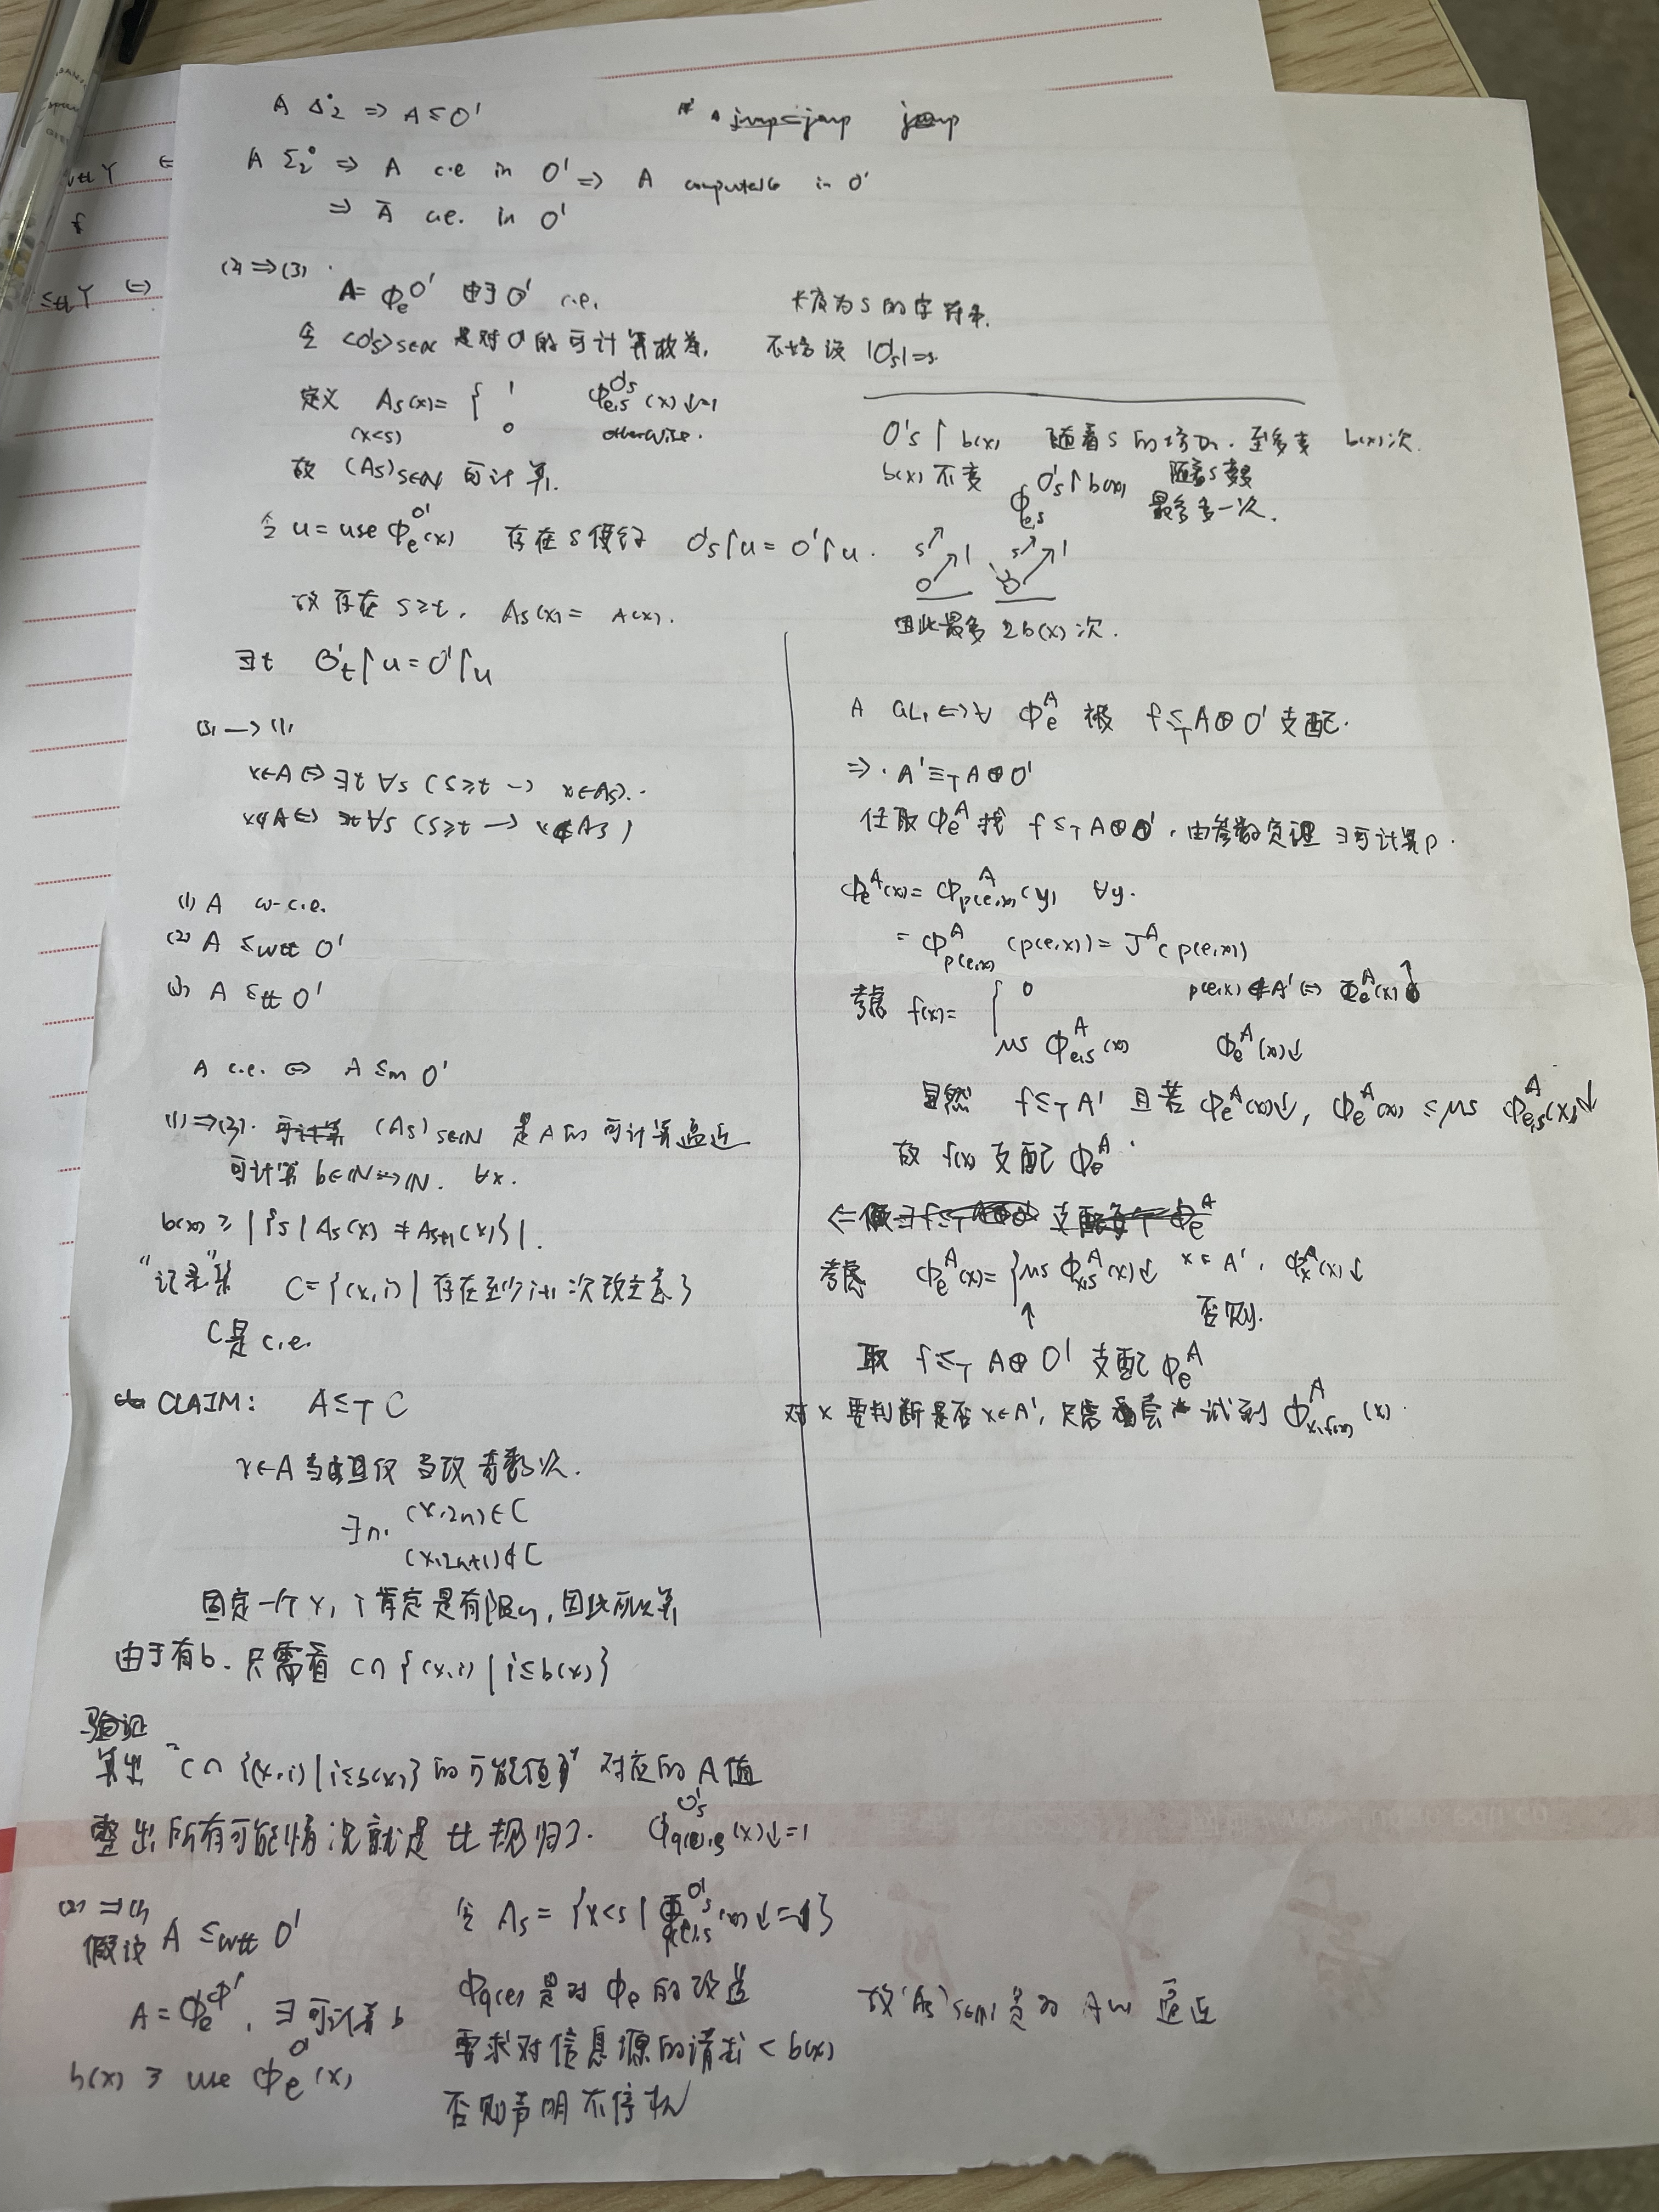
\includegraphics[width=.5\textwidth]{../images/AnIntroductionToAlgebraicTopology/1.png}
\label{}
\end{figure}
If \(G\) is the graph of \(f\) and \(\Delta\) is the graph of the identity function, then we must prove
that \(G\cap\Delta\neq\emptyset\). The idea is to use a connectness argument to show that every path in \(D^1\times D^1\)
from \(a\) to \(b\) must cross \(\Delta\).

Since \(f\) is continuous, \(G=\{(x,f(x)):x\in D^1\}\) is connected (continuous image of connected
space is connected). Define \(A=\{(x,f(x)):f(x)>x\}\)  and \(B=\{(x,f(x)):f(x)<x\}\). Note
that \(a\in A\) and \(b\in B\), so that \(A\neq\emptyset\) and \(B\neq\emptyset\). If \(G\cap\Delta=\emptyset\), then \(G\) is the disjoint
union of \(A\) and \(B\).
\end{proof}


\begin{theorem}[Brouwer fixed point theorem]
If \(f:D^n\to D^n\) is continuous, then there exists \(x\in D^n\) with \(f(x)=x\)
\end{theorem}

\section{Categories and Functors}
\label{sec:org5fe485b}
\begin{definition}[]
A category \(\calc\) consists of three ingredients: a class of \textbf{objects}, \(\obj\calc\); sets of
\textbf{morphisms} \(\Hom(A,B)\), one for every ordered pair \(A,B\in\obj\calc\);
\textbf{composition} \(\Hom(A,B)\times\Hom(B,C)\to\Hom(A,C)\), denoted by \((f,g)\to g\circ f\), for
every \(A,B,C\in\obj\calc\) satisfying the following axioms
\begin{enumerate}
\item the family of \(\Hom(A,B)\)'s is pairwise disjoint
\item composition is associative when defined
\item for each \(A\in\obj\calc\) there exists an identity \(1_A\in\Hom(A,A)\) satisfying \(1_A\circ f=f\) for
every \(f\in\Hom(B,A)\), all \(B\in\obj\calc\) and \(g\circ 1_A=g\) for every \(g\in\Hom(A,C)\), all \(C\in\obj\calc\)
\end{enumerate}
\end{definition}

\begin{definition}[]
Let \(\calc\) and \(\cala\) be categories with \(\obj\calc\subset\obj\cala\). If \(A,B\in\obj\calc\), let's denote the two
possible Hom sets by \(\Hom_{\calc}(A,B)\) and \(\Hom_{\cala}(A,B)\). Then \(\calc\) is a \textbf{subcategory}
of \(\cala\) if \(\Hom_{\calc}(A,B)\subset\Hom_{\cala}(A,B)\) for all \(A,B\in\obj\calc\) and if composition in \(\calc\) is
the same as composition in \(\cala\)
\end{definition}

\begin{examplle}[]
\(\calc=\Top^{2}\). here \(\obj\calc\) consists of all ordered pairs \((X,A)\) where \(X\) is a topological
space and \(A\) is a subspace of \(X\). A morphism \(f:(X,A)\to(Y,B)\) is an ordered
pair \((f,f')\) where \(f:X\to Y\) is continuous and \(fi=jf'\) (where \(i\) and \(j\) are
inclusions)
\begin{center}
\begin{tikzcd}
A\arrow[r,hookrightarrow,"i"]\arrow[d,"f'"']&X\arrow[d,"f"]\\
B\arrow[r,hookrightarrow,"j"']&Y
\end{tikzcd}
\end{center}
and composition is coordinatewise. \(\Top^2\) is called the category of \textbf{pairs} (of topological spaces)
\end{examplle}

\begin{examplle}[]
\(\calc=\Top_*\). Here \(\obj\calc\) consists of all ordered pairs \((X,x_0)\) where \(X\) is a
topological space and \(x_0\) is a point of \(X\). \(\Top_*\) is a subcategory of \(\Top^2\) and
it is called the category of \textbf{pointed spaces}; \(x_0\) is called the \textbf{basepoint} of \((X,x_0)\) and
morphisms are called \textbf{pointed maps} (or \textbf{basepoint preserving maps}). The category \(\Sets_*\) of
pointed sets is defined similarly
\end{examplle}

\begin{exercise}
\label{ex0.7}
Let \(f\in\Hom(A,B)\) be a morphism in a category \(\calc\). If \(f\) has a left inverse \(g\)
(\(g\in\Hom(B,A)\)$\backslash$ and \(g\circ f=1_A\)) and a right inverse \(h\) (\(h\in\Hom(B,A)\) and \(f\circ h=1_B\)),
then \(g=h\)
\end{exercise}

\begin{exercise}
\label{ex0.9}
A set \(X\) is called \textbf{quasi-ordered} (or \textbf{pre-ordered}) if \(X\) has a transitive and reflexive
relation \(\le\) (such a set is partially ordered if \(\le\) is antisymmetric). Prove that the
following construction gives a category \(\calc\). Define \(\obj\calc=X\), if \(x,y\in X\)
and \(x\not\le y\), define \(\Hom(x,y)=\emptyset\); if \(x\le y\), define \(\Hom(x,y)\) to be a set with
exactly one element, denoted by \(i_y^x\); if \(x\le y\le z\) define composition by \(i_z^y\circ i_y^x=i_z^x\)
\end{exercise}

\begin{exercise}
\label{ex0.10}
Let \(G\) be a \textbf{monoid}, that is, a semigroup with 1. Show that the following gives a
category \(\calc\). Let \(\obj\calc\) have exactly one element, denoted by \textbf{; define $\backslash$(\Hom(},*)=G$\backslash$) and
define composition \(G\times G\to G\) as the given multiplication in \(G\)
\end{exercise}

\begin{definition}[]
A \textbf{diagram} in a category \(\calc\) is a directed graph whose vertices are labeled by objects of \(\calc\) and
whose directed edges are labeled by morphisms in \(\calc\). A \textbf{commutative diagram} in \(\calc\) is a diagram in
which, for each pair of vertices, every two paths (composites) between them are equal as
morphisms.
\end{definition}

\begin{exercise}
\label{ex0.12}
Given a category \(\calc\), shows that the following construction gives a category \(\calm\). First, an
object of \(\calm\) is a morphism of \(\calc\). Next, if \(f,g\in\obj\calm\), say \(f:A\to B\) and \(g:C\to D\),
then a morphism in \(\calm\) is an ordered pair \((h,k)\) of morphisms in \(\calc\) s.t. the diagram
\begin{center}\begin{tikzcd}
A\arrow[r,"f"]\arrow[d,"h"']&B\arrow[d,"k"]\\
C\arrow[r,"g"']&D
\end{tikzcd}\end{center}
commutes. Define composition coordinatewise
\begin{equation*}
(h',k')\circ(h,k)=(h'\circ h,k'\circ k)
\end{equation*}
\end{exercise}

\index{congruence}
\begin{definition}[]
A \textbf{congruence} on a category \(\calc\) is an equivalence relation \(\sim\) on the
class \(\bigcup_{(A,B)}\Hom(A,B)\) of all morphisms in \(\calc\) s.t.
\begin{enumerate}
\item \(f\in\Hom(A,B)\) and \(f\sim f'\) implies \(f'\in\Hom(A,B)\)
\item \(f\sim f'\), \(g\sim g'\) and the composite \(g\circ f\) exists imply that
\begin{equation*}
g\circ f\sim g'\circ f'
\end{equation*}
\end{enumerate}
\end{definition}

\begin{theorem}[]
\label{thm0.4}
Let \(\calc\) be a category with congruence \(\sim\) and let \([f]\) denote the equivalence class of a
morphism \(f\). Define \(\calc'\) as follows
\begin{align*}
\obj\calc'&=\obj\calc\\
\Hom_{\calc'}(A,B)&=\{[f]:f\in\Hom_{\calc}(A,B)\}\\
[g]\circ[f]&=[g\circ f]
\end{align*}
Then \(\calc'\) is a category
\end{theorem}

\begin{proof}
Property 1 in the definition of congruence shows that \(\sim\) partitions each set \(\Hom_{\calc}(A,B)\)
and this implies that \(\Hom_{\calc'}(A,B)\) is a set; moreover, the family of these sets is pairwise
disjoint. Property 2 in the definition of congruence shows that composition in \(\calc'\) is
well. \(\calc'\) is associative and \([1_A]\) is the identity is not hard
\end{proof}

The category \(\calc'\) is called a \textbf{quotient category} of \(\calc\); one usually
denotes \(\Hom_{\calc'}(A,B)\) by \([A,B]\)

\begin{exercise}
\label{ex0.14}
Let \(G\) be a group and let \(\calc\) be the one-object category it
defines: \(\obj\calc=\{*\}\), \(\Hom( *, *)=G\) and composition is the group operation. If \(H\) is a
normal subgroup of \(G\), define \(x\sim y\) to mean \(xy^{-1}\in H\). Show that \(\sim\) is a congruence
on \(\calc\) and that \([*, *]=G/H\) in the corresponding quotient category
\end{exercise}

\index{functor}
\begin{definition}[]
If \(\cala\) and \(\calc\) are categories, a \textbf{functor} \(T:\cala\to\calc\) is a function, that is,
\begin{enumerate}
\item \(A\in\obj\cala\) implies \(TA\in\obj\calc\)
\item if \(f:A\to A'\) is a morphism in \(\cala\), then \(Tf:TA\to TA'\) is a morphism in \(\calc\)
\item if \(f,g\) are morphisms in \(\cala\) for which \(g\circ f\) is defined, then
\begin{equation*}
T(g\circ f)=(Tg)\circ (Tf)
\end{equation*}
\item \(T(1_A)=1_{TA}\) for every \(A\in\obj\cala\)
\end{enumerate}
\end{definition}

\begin{examplle}[]
If \(\calc\) is a category, the \textbf{identity functor} \(J:\calc\to\calc\) is defined by \(JA=A\) for every
object \(A\) and \(Jf=f\) for every morphism
\end{examplle}

\begin{examplle}[]
If \(M\) is a fixed topological space, Then \(T_m:\Top\to\Top\) is a functor,
where \(T_M(X)=X\times M\) and if \(f:X\to Y\) is continuous, then \(T_M(f):X\times M\to Y\times M\) is defined by
\((x,m)\mapsto(f(x),m)\)
\end{examplle}

\begin{examplle}[]
Fix an object \(A\) in category \(\calc\). Then \(\Hom(A,-):\calc\to\Sets\) is a functor assigning to each
object \(B\) the set \(\Hom(A,B)\) and to each morphism \(f:B\to B'\) the \textbf{induced
map} \(\Hom(A,f):\Hom(A,B)\to\Hom(A,B')\) defined by \(g\mapsto f\circ g\). One usually denotes the induced
map \(\Hom(A,f)\) by \(f_*\)
\end{examplle}

Functors as just defined are also called \textbf{covariant functors} to distinguish them from
\textbf{contravariant functors} that reverse the direction of arrows. Thus the functor of the example  is
sometimes called a \textbf{covariant Hom functor}.

\begin{definition}[]
if \(\cala\) and \(\calc\) are categories, a \textbf{contravariant functor} \(S:\cala\to\calc\) is a function that
\begin{enumerate}
\item \(A\in\obj\cala\) implies \(SA\in\obj\calc\)
\item if \(f:A\to A'\) is a morphism in \(\calc\), then \(Sf:SA'\to SA\) is a morphism in \(\calc\)
\item if \(f,g\) are morphisms in \(\cala\) for which \(g\circ f\) is defined, then
\begin{equation*}
S(g\circ f)=S(f)\circ S(g)
\end{equation*}
\item \(S(1_A)=1_{SA}\) for every \(A\in\obj\cala\)
\end{enumerate}
\end{definition}

\begin{examplle}[]
Fix an object \(B\) in a category \(\calc\). Then \(\Hom(-,B):\calc\to\Sets\) is a contravariant functor
assigning to each object \(A\) the set \(\Hom(A,B)\) and to each morphism \(g:A\to A'\) the
\textbf{induced map} \(\Hom(g,B):\Hom(A',B)\to\Hom(A,B)\) defined by \(h\mapsto h\circ g\). One usually denotes the
induced map \(\Hom(g,B)\) by \(g^*\); \(\Hom(-,B)\) is called a \textbf{contravariant Hom functor}
\end{examplle}

\begin{definition}[]
An \textbf{equivalence} in a category \(\calc\) is a morphism \(f:A\to B\) for which there exists a
morphism \(g:B\to A\) with \(f\circ g=1_B\) and \(g\circ f=1_A\)
\end{definition}

\begin{theorem}[]
If \(\cala\) and \(\calc\) are categories and \(T:\cala\to\calc\) is a functor of either variance, then \(f\) an
equivalence in \(\cala\) implies that \(Tf\) is an equivalence in \(\calc\)
\end{theorem}

\begin{exercise}
\label{ex0.17}
Let \(\calc\) and \(\cala\) be categories, let \(\sim\) be a congruence on \(\calc\). If \(T:\calc\to\cala\) is a functor
with \(T(f)=T(g)\) whenever \(f\sim g\), then \(T\) defines a functor \(T':\calc'\to\cala\) (where \(\calc'\) is
the quotient category) by \(T'(X)=T(X)\) for every object \(X\) and \(T'([f])=T(f)\) for every
morphism \(f\).
\end{exercise}

\begin{exercise}
\label{ex0.20}
\begin{enumerate}
\item if \(X\) is a topological space,  show that \(C(X)\), the set of all continuous real-valued
functions on \(X\), is a commutative ring with 1 under pointwise operations
\begin{equation*}
f+g:x\mapsto f(x)+g(x)\quad\text{ and }\quad f\cdot g\mapsto f(x)g(x)
\end{equation*}
for all \(x\in X\)
\item show that \(X\mapsto C(X)\) gives a (contravariant) functor \(\Top\to\Rings\)
\end{enumerate}
\end{exercise}

\begin{proof}
\begin{enumerate}
\setcounter{enumi}{1}
\item From exercise \ref{ex0.12}
\end{enumerate}
\end{proof}


\section{Some Basic Topological Notions}
\label{sec:org0dd8dd0}

\subsection{Homotopy}
\label{sec:orgbf0fe41}
\begin{definition}[]
If \(X\) and \(Y\) are spaces and if \(f_0,f_1\) are continuous maps from \(X\) to \(Y\),
then \(f_0\) is \textbf{homotopic} to \(f_1\), denoted by \(f_0\simeq f_1\) if there is a continuous
map \(F:X\times\bI\to Y\) with
\begin{equation*}
F(x,0)=f_0(x) \quad\text{ and }\quad F(x,1)=f_1(x) \quad\text{for all }x\in X
\end{equation*}
Such a map \(F\) is called a \textbf{homotopy}, written as \(F:f_0\simeq f_1\)
\end{definition}

If \(f_t:X\to Y\) is defined by \(f_t(x)=F(x,t)\), then a homotopy \(F\) gives a one-parameter
family of continuous maps deforming \(f_0\) into \(f_1\)

\begin{lemma}[Gluing lemma]
Assume that a space \(X\) is a finite union of closed subsets \(X=\bigcup_{i=1}^nX_i\). If, for some
space \(Y\), there are continuous maps \(f_i:X_i\to Y\) that agree on overlaps
(\(f_i|X_i\cap X_j=f_j|X_i\cap X_j\) for all \(i,j\)), then there exists a unique continuous \(f:X\to Y\)
with \(f|X_i=f_i\) for all \(i\)
\end{lemma}

\begin{proof}
If \(C\) is closed in \(Y\), then
\begin{align*}
f^{-1}(C)&=X\cap f^{-1}(C)=(\bigcup X_i)\cap f^{-1}(C)\\
&=\bigcup (X_i\cap f^{-1}(C))\\
&=\bigcup (X_i\cap f_i^{-1}(C))=\bigcup f_i^{-1}(C)
\end{align*}
Since each \(f_i\) is continuous, \(f_i^{-1}(C)\) is closed in \(X_i\). Since \(X_i\) is closed
in \(X\), \(f_i^{-1}(C)\) is closed in \(X\), therefore \(f^{-1}(C)\) is closed in \(X\) and \(f\)
is continuous
\end{proof}

\begin{lemma}[Gluing Lemma]
Assume that a space \(X\) has a (possibly infinite) open cover \(X=\bigcup X_i\). If for some
space \(Y\), there are continuous maps \(f_i:X_i\to Y\) that agree on overlaps, then there exists a
unique continuous \(f:X\to Y\) with \(f|X_i=f_i\) for all \(i\)
\end{lemma}

\begin{theorem}[]
Homotopy is an equivalence relation on the set of all continuous maps \(X\to Y\)
\end{theorem}

\begin{proof}
\emph{Reflexivity}. If \(f:X\to Y\), define \(F:X\times\bI\to Y\) by \(F(x,t)=f(x)\) for all \(x\in X\) and \(t\in\bI\);
clearly \(F:f\simeq f\)

\emph{Symmetry}: Assume that \(f\simeq g\), so there is a continuous \(F:X\times\bI\to Y\) with \(F(x,0)=f(x)\)
and \(F(x,1)=g(x)\) for all \(x\in X\). Define \(G:X\times\bI\to Y\) by \(G(x,t)=F(x,1-t)\), and note
that \(G:g\simeq f\).

\emph{Transivity}: assume that \(F:f\simeq g\) and \(G:g\simeq h\). Define \(H:X\times\bI\to Y\) by
\begin{equation*}
H(x,t)=
\begin{cases}
F(x,2t)&0\le t\le 1/2\\
G(x,2t-1)&1/2\le t\le 1
\end{cases}
\end{equation*}
Because these functions agree on the overlap \(\{(x,1/2):x\in X\}\), the gluing lemma shows
that \(H\) is continuous. Therefore \(H:f\simeq h\)
\end{proof}

\begin{definition}[]
If \(f:X\to Y\) is continuous, its \textbf{homotopy class} is the equivalence class
\begin{equation*}
[f]=\{\text{continuous }g:X\to Y:g\simeq f\}
\end{equation*}
The family of all such homotopy classes is denoted by \([X,Y]\)
\end{definition}

\begin{theorem}[]
Let \(f_i:X\to Y\) and \(g_i:Y\to Z\), for \(i=0,1\), be continuous. If \(f_0\simeq f_1\) and \(g_0\simeq g_1\),
then \(g_0\circ f_0\simeq g_1\circ f_1\); that is, \([g_0\circ f_0]=[g_1\circ f_1]\)
\end{theorem}

\begin{proof}
Let \(F:f_0\simeq f_1\) and \(G:g_0\simeq g_1\) be homotopies. First, we show that
\begin{equation*}
g_0\circ f_0\simeq g_1\circ f_0
\end{equation*}
Define \(H:X\times\bI\to Z\) by \(H(x,t)=G(f_0(x),t)\). Clearly, \(H\) is continuous;
moreover, \(H(x,0)=G(f_0(x),0)=g_0(f_0(x))\) and \(H(x,1)=G(f_0(x),1)=g_1(f_0(x))\). Now observe
that
\begin{equation*}
K:g_1\circ f_0\sim g_1\circ f_1
\end{equation*}
where \(K:X\times\bI\to Z\) is the composite \(g_1\circ F\). Now use the transitivity of the homotopy relation,
we have \(g_0\circ f_0\simeq g_1\circ f_1\)
\end{proof}

\begin{corollary}[]
Homotopy is a congruence on the category \(\Top\).
\end{corollary}

It follows from Theorem \ref{thm0.4} that there is a quotient category whose objects are
topological spaces \(X\), whose Hom sets are \(\Hom(X,Y)=[X,Y]\) and whose composition
is \([g]\circ[f]=[g\circ f]\)

\begin{definition}[]
The quotient category just described is called the \textbf{homotopy category}, and it is denoted by
\(\hTop\)
\end{definition}

All the functors \(T:\Top\to\cala\) that we shall construct, where \(\cala\) is some ``algebraic'' category
(e.g. \(\Ab\), \(\Groups\), \(\Rings\)) will have the property that \(f\simeq g\)
implies \(T(f)=T(g)\). This fact, aside from a natural wish to identify homotopic maps, makes
homotopy valuable, \emph{beacause it guarantees that the algebraic problem in \(\cala\) arising from a}
\emph{topological problem via \(T\) is simpler than the original problem}

\begin{definition}[]
A continuous map \(f:X\to X\) is a \textbf{homotopy equivalence} if there is a continuous map \(g:Y\to X\)
with \(g\circ f\simeq 1_X\) and \(f\circ g\simeq 1_Y\). Two spaces \(X\) and \(Y\) have the \textbf{same homotopy type} if
there is a homotopy equivalence \(f:X\to Y\)
\end{definition}

\(f\) is a homotopy equivalence iff \([f]\in[X,Y]\) is an equivalence in \(\hTop\). (\label{Problem1})

\begin{definition}[]
Let \(X\) and \(Y\) be spaces, and let \(y_0\in Y\). The \textbf{constant map} at \(y_0\) is the
function \(c:X\to Y\) with \(c(x)=y_0\) for all \(x\in X\). A continuous map \(f:X\to Y\) is
\textbf{nullhomotopic} if there is a constant map \(c:X\to Y\) with \(f\simeq c\)
\end{definition}

\begin{theorem}[]
\label{thm1.5}
Let \(\C\) denote the complex numbers, let \(\Sigma_\rho\subset\C\approx\R^2\) denote the circle with center at the origin
0 and radius \(\rho\), and let \(f_\rho^n:\Sigma_\rho\to\C-\{0\}\) denote the restriction to \(\Sigma^\rho\) of \(z\mapsto z^n\). If none
of the maps \(f_\rho^n\) is nullhomotopic (\(n\ge 1\) and \(\rho>0\)) then the fundamental theorem of
algebra is true (i.e., every nonconstant complex polynomial has a complex root)
\end{theorem}

\begin{proof}
Consider the polynomial with complex coefficients
\begin{equation*}
g(z)=z^n+a_{n-1}z^{n-1}+\dots+a_1z+a_0
\end{equation*}
Choose \(\rho>\max\{1,\sum_{i=1}^{n-1}\abs{a_i}\}\) and define \(F:\Sigma_\rho\times\bI\to\C\)
\begin{equation*}
F(z,t)=z^n+\sum_{i=0}^{n-1}(1-t)a_iz^i
\end{equation*}
It's obvious that \(F:g|\Sigma_\rho\simeq f_\rho^n\) if we can show that the image of \(F\) is contained
in \(\C-\{0\}\). that is, \(F(z,t)\neq0\). If, on the contrary, \(F(z,t)=0\)  for some \(t\in\bI\) and
some \(z\) with \(\abs{z}=\rho\), then \(z^n=-\sum_{i=0}^{n-1}(1-t)a_iz^i\). The triangle inequality gives
\begin{equation*}
\rho^n\le\sum_{i=0}^{n-1}(1-t)\abs{a_i}\rho^i\le\sum_{i=0}^{n-1}\abs{a_i}\rho^i\le\left(\sum_{i=0}^{n-1}\abs{a_i}\right)\rho^{n-1}
\end{equation*}
for \(\rho>1\) implies that \(\rho^i\le\rho^{n-1}\). Canceling \(\rho^{n-1}\) gives \(\rho\le\sum_{i=0}^{n-1}\abs{a_i}\),
a contradiction.

Assume now that \(g\) has no complex roots. Define \(G:\Sigma_\rho\times\bI\to\C-\{0\}\) by
\(G(z,t)=g((1-t)z)\). (Since \(g\) has no roots, the values of \(G\) do lie in \(\C-\{0\}\))
Visibly, \(G:g|\Sigma_\rho\simeq k\), where \(k\) is the constant function at \(a_0\). Therefore \(g|\Sigma_\rho\) is
nullhomotopic and by transitivity, \(f_\rho^n\) is nullhomotopic, contradicting the hypothesis.
\end{proof}

A common problem involves extending a map \(f:X\to Z\) to a larger space \(Y\); the picture is
\begin{center}\begin{tikzcd}
Y\arrow[dr,dashed,"g"]\\
X\arrow[u,hookrightarrow]\arrow[r,"f"']&Z
\end{tikzcd}\end{center}
Homotopy itself raises such a problem: if \(f_0,f_1:X\to Z\) then \(f_0\simeq f_1\) if we can
extend \(f_0\cup f_1:X\times\{0\}\cup X\times\{1\}\to Z\) to all of \(X\times I\)


\section{Problem}
\label{sec:orgaf7b91d}
\label{Problem1}

\section{Index}
\label{sec:orgd79a4c8}
\renewcommand{\indexname}{}
\printindex
\end{document}
